%
% relazione_es0.tex
%
% Copyright (C) 2016 frnmst (Franco Masotti) <franco.masotti@student.unife.it>
%                    dannylessio (Danny Lessio)
%
% This file is part of networks-lab.
%
% networks-lab is free software: you can redistribute it and/or modify
% it under the terms of the GNU General Public License as published by
% the Free Software Foundation, either version 3 of the License, or
% (at your option) any later version.
%
% networks-lab is distributed in the hope that it will be useful,
% but WITHOUT ANY WARRANTY; without even the implied warranty of
% MERCHANTABILITY or FITNESS FOR A PARTICULAR PURPOSE.  See the
% GNU General Public License for more details.
%
% You should have received a copy of the GNU General Public License
% along with networks-lab.  If not, see <http://www.gnu.org/licenses/>.
%

\makeatletter
\def\blfootnote{\xdef\@thefnmark{}\@footnotetext}
\makeatother

\documentclass[11pt, a4paper, oneside]{article}
	\usepackage{setspace} % packets
	\usepackage{graphicx} % pictures
	\usepackage[gen]{eurosym} % euro symbol
	\usepackage{float} % used for H option in pictures
	\singlespacing % interlinea singolo
	\title{Relazione esercitazione 1 Laboratorio di reti}
	\author{Franco Masotti \and Danny Lessio}
	\date{March 9, 2015}
\begin{document}
	\maketitle
	\tableofcontents
	\listoffigures
	\listoftables
	\newpage
    \footnotetext{networks-lab  Copyright (C) 2016  frnmst (Franco Masotti), 
dannylessio (Danny Lessio).  This document comes with ABSOLUTELY NO WARRANTY.
This is free software, and you are welcome to redistribute it 
under certain conditions; see LICENSE file for details.}
	\part{Scelte di progetto}
		\section{Scelte generali}
			\par
			La scelta del centro stella \'e ricaduta nell'edificio centrale della facolt\'a in quanto si trova in una posizione strategica dalla quale si possono raggiungere facilmente, in fibra, gli switch di piano sia della parte nuova sia della parte vecchia. Questa stanza \'e climatizzata per mantenere una temperatura costante adatta alle macchine. 
			\par
			Abbiamo deciso di utilizzare un collegamento di tipo fibra multimodale (\texttt{SFP+}) 10Gbit Ethernet per collegare lo switch centro stella agli switch di piano. In questo modo gli switch di piano si possono posizionare anche svariate decine di metri dallo switch centro stella in totale sicurezza. Inoltre questo garantisce di avere un'ottima banda anche per gli anni a venire.
			\par
			Per collegare gli switch di piano agli switch locali (dei laboratori o uffici) o a degli access point o prese ethernet, abbiamo utilizzato dei cavi in rame cat 6a (fino a 10Gbps) STP per evitare interferenze che potrebbero degradare le prestazioni.
			\par
			Lo switch del centro stella è collegato al router con un cavo in fibra multimodale, in quanto pi\'u veloce ed affidabile di un cavo in rame ed anche perch\'e lo switch ha 32 porte in fibra di cui meno della met\'a occupata dagli switch di piano.
			\par
			Per ottimizzare i costi abbiamo usato il numero minimo di canalette posizionando gli elementi (quali access point, switch e prese ethernet) in posizioni strategiche.
			\par
			Nelle zone di edificio in cui la sorgente dei cavi in rame (cio\'e lo switch di piano) e la destinazione (un qualunque elemento attivo o passivo della rete) fossero troppo distanti tra loro a causa della dispersione del segnale, abbiamo usato uno switch Gbit Ethernet con porte in rame, posizionato ad una distanza di sicurezza dallo switch di piano.
			\par
			La struttura ha una copertura totale in wifi di ultima generazione in dual band (anche \texttt{ac}) cos\'i da sfruttare appieno i collegamenti con gli switch.
		\section{Apparecchiature}
			\par
			In generale gli apparati di rete sono \texttt{Cisco} poich\'e sono modulari (in particolare gli switch) e quindi \'e possibile acquistare moduli in futuro senza cambiare totalmente l'apparecchio.
			\par
			Per replicare porte ethernet in zone in cui si rendono necessari molti collegamenti (ad es. laboratori di informatica), abbiamo utilizzato degli switch gigabit Ethernet in rame \texttt{HP} con 48 porte, collegati agli switch di piano.
			\par
			Il gruppo di continuit\'a (\texttt{UPS}) dell'\texttt{APC} garantisce alimentazione alle apparechiature di rete principali, per un periodo limitato di tempo anche sotto forte carico.
				
	\newpage
	\part{Planimetrie}
		\section{Legenda}
			\begin{figure}[H]
				\caption{Legenda}
				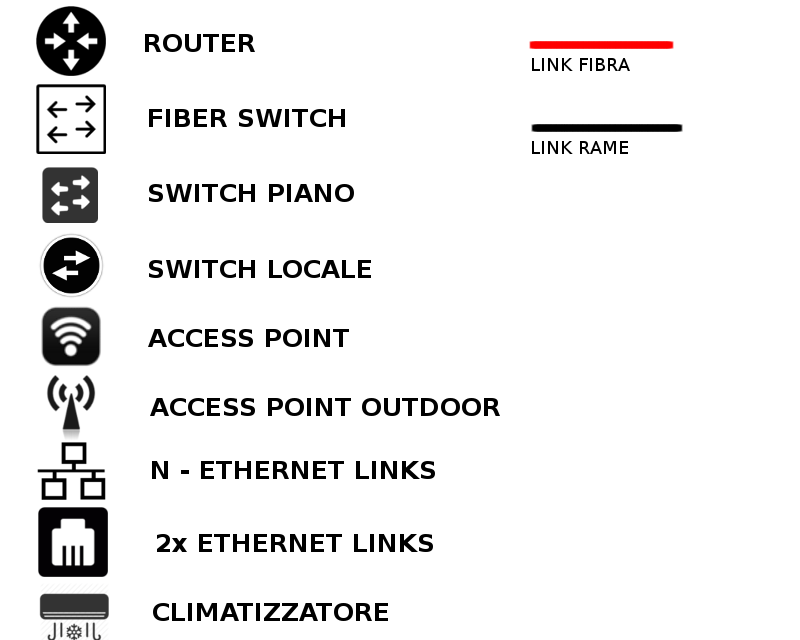
\includegraphics[scale=0.5]{legenda.png}
			\end{figure}
			\newpage
		\section{Vecchio edificio}
			\begin{figure}[H]
				\caption{Piano terra, vecchio edificio}
				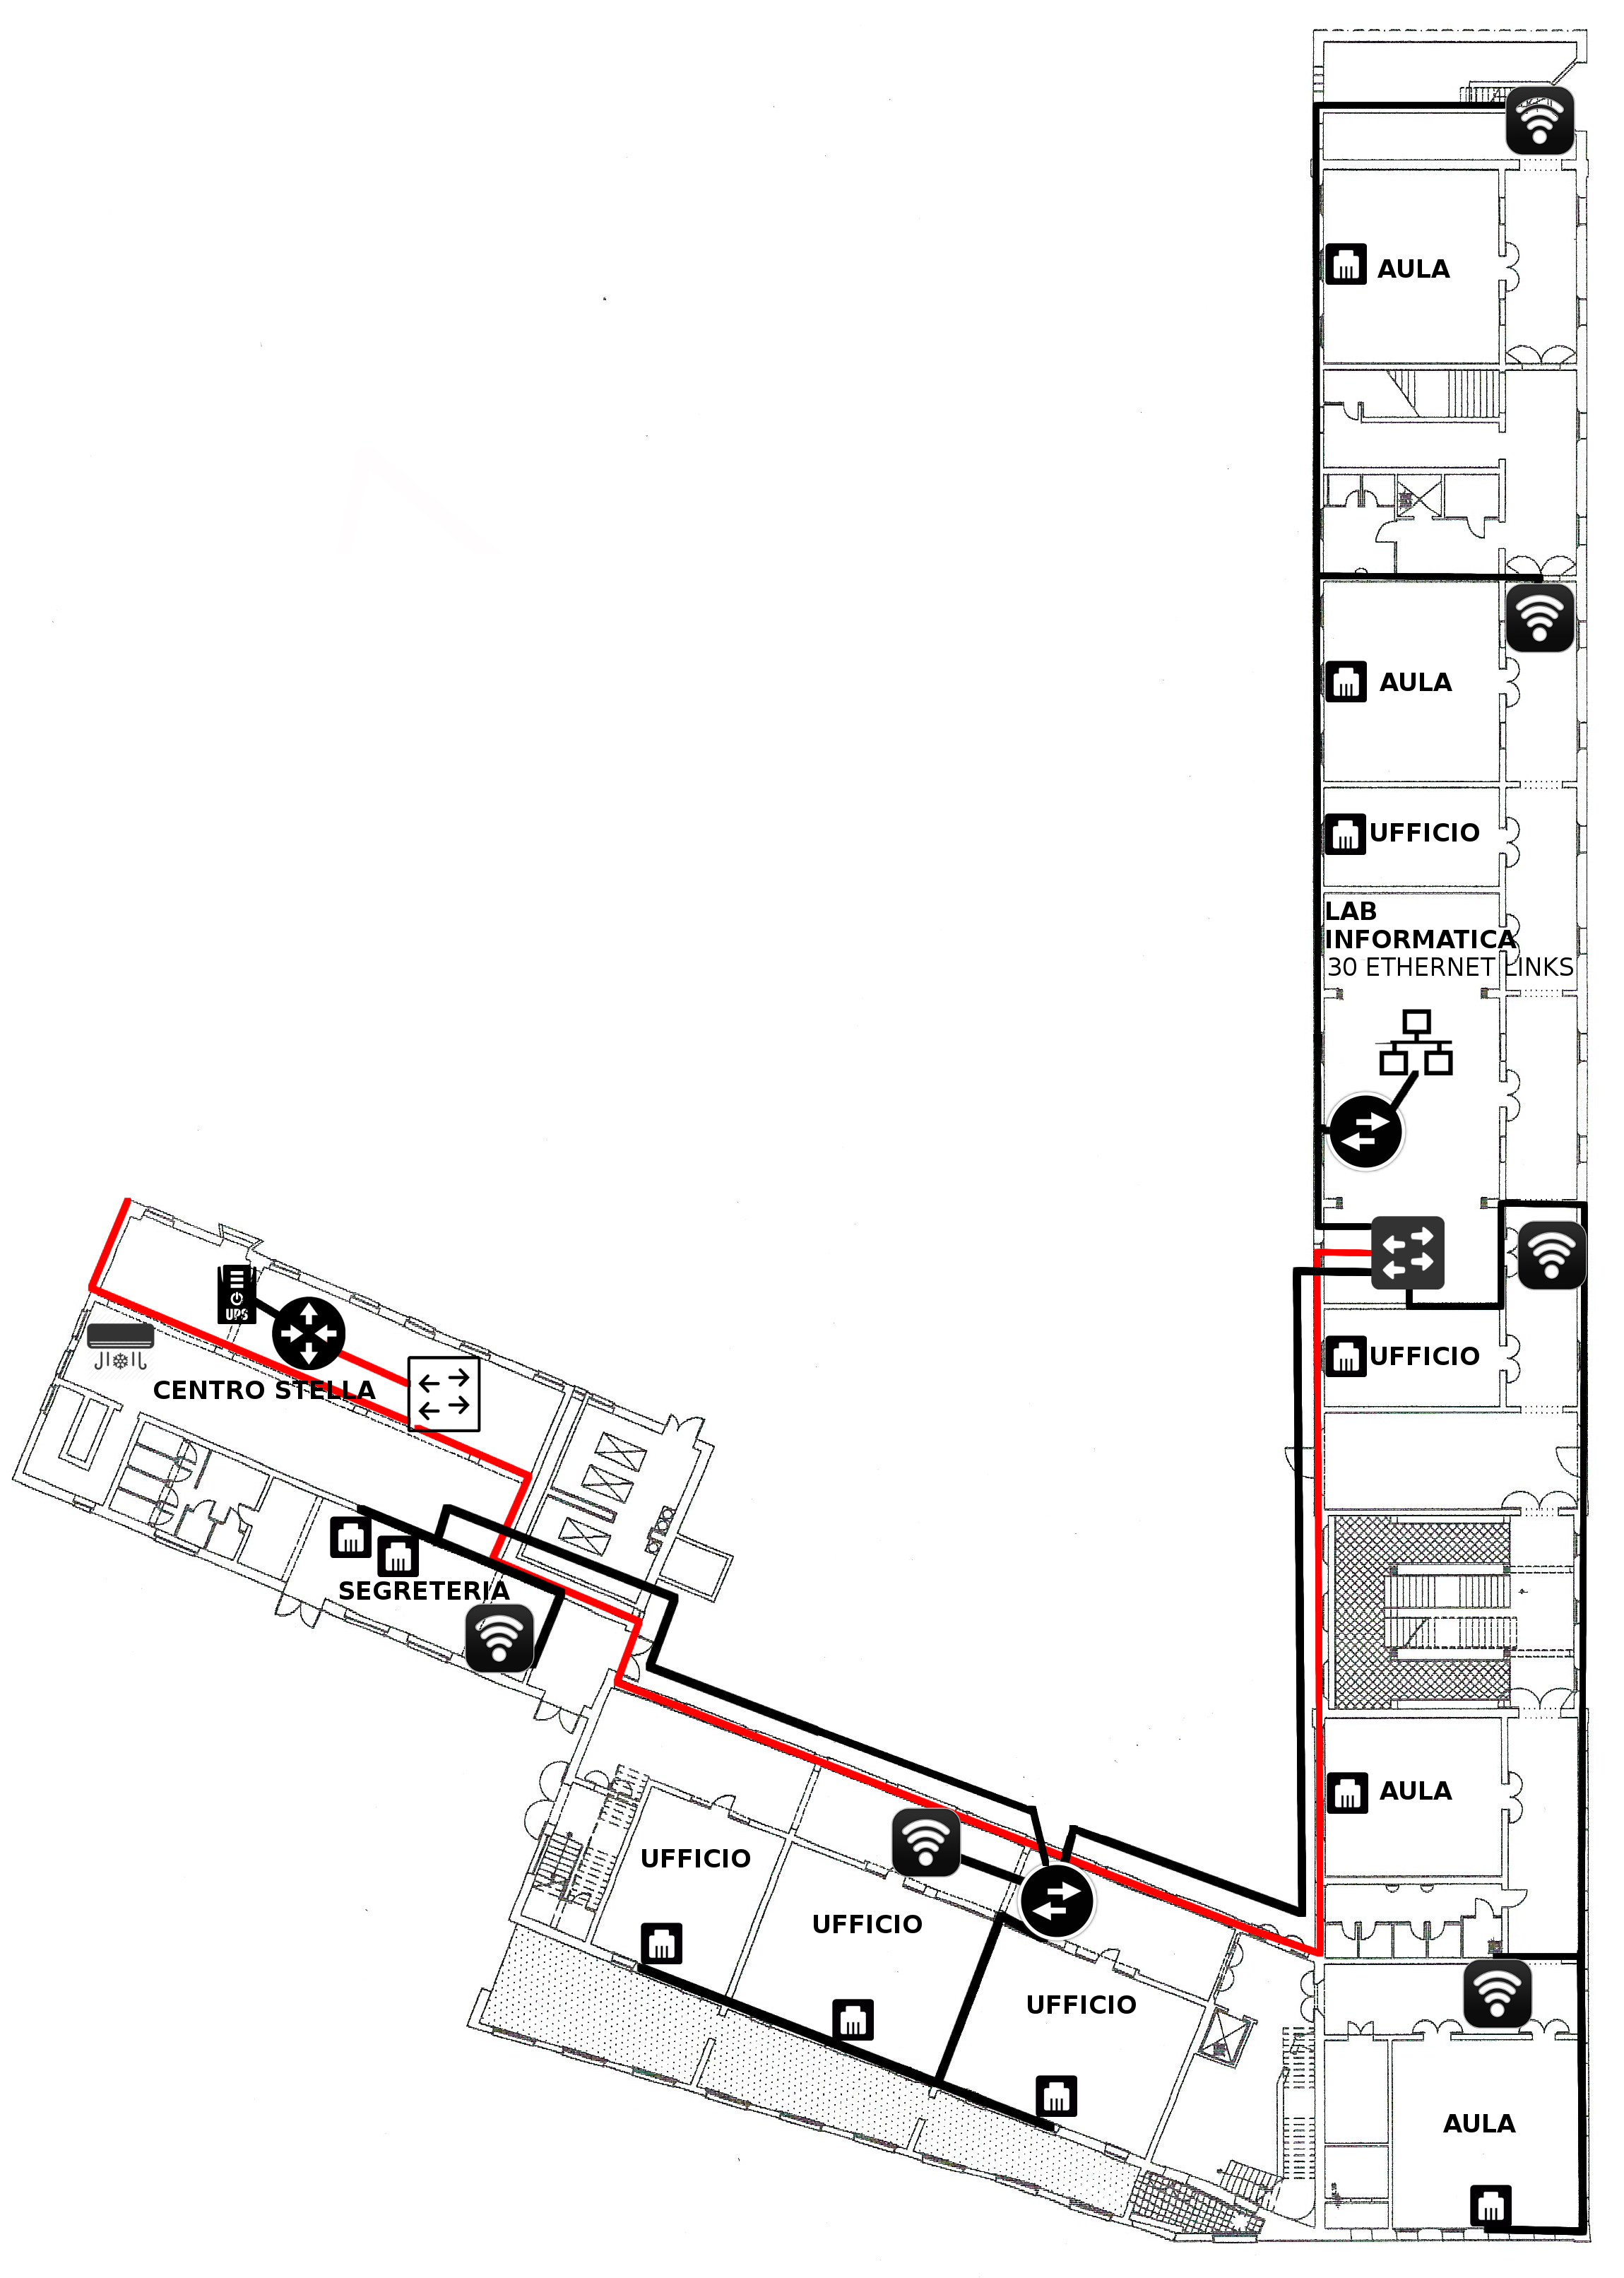
\includegraphics[scale=0.2]{architecture-001.png}
			\end{figure}
			\begin{figure}[H]
				\caption{Primo piano, vecchio edificio}
				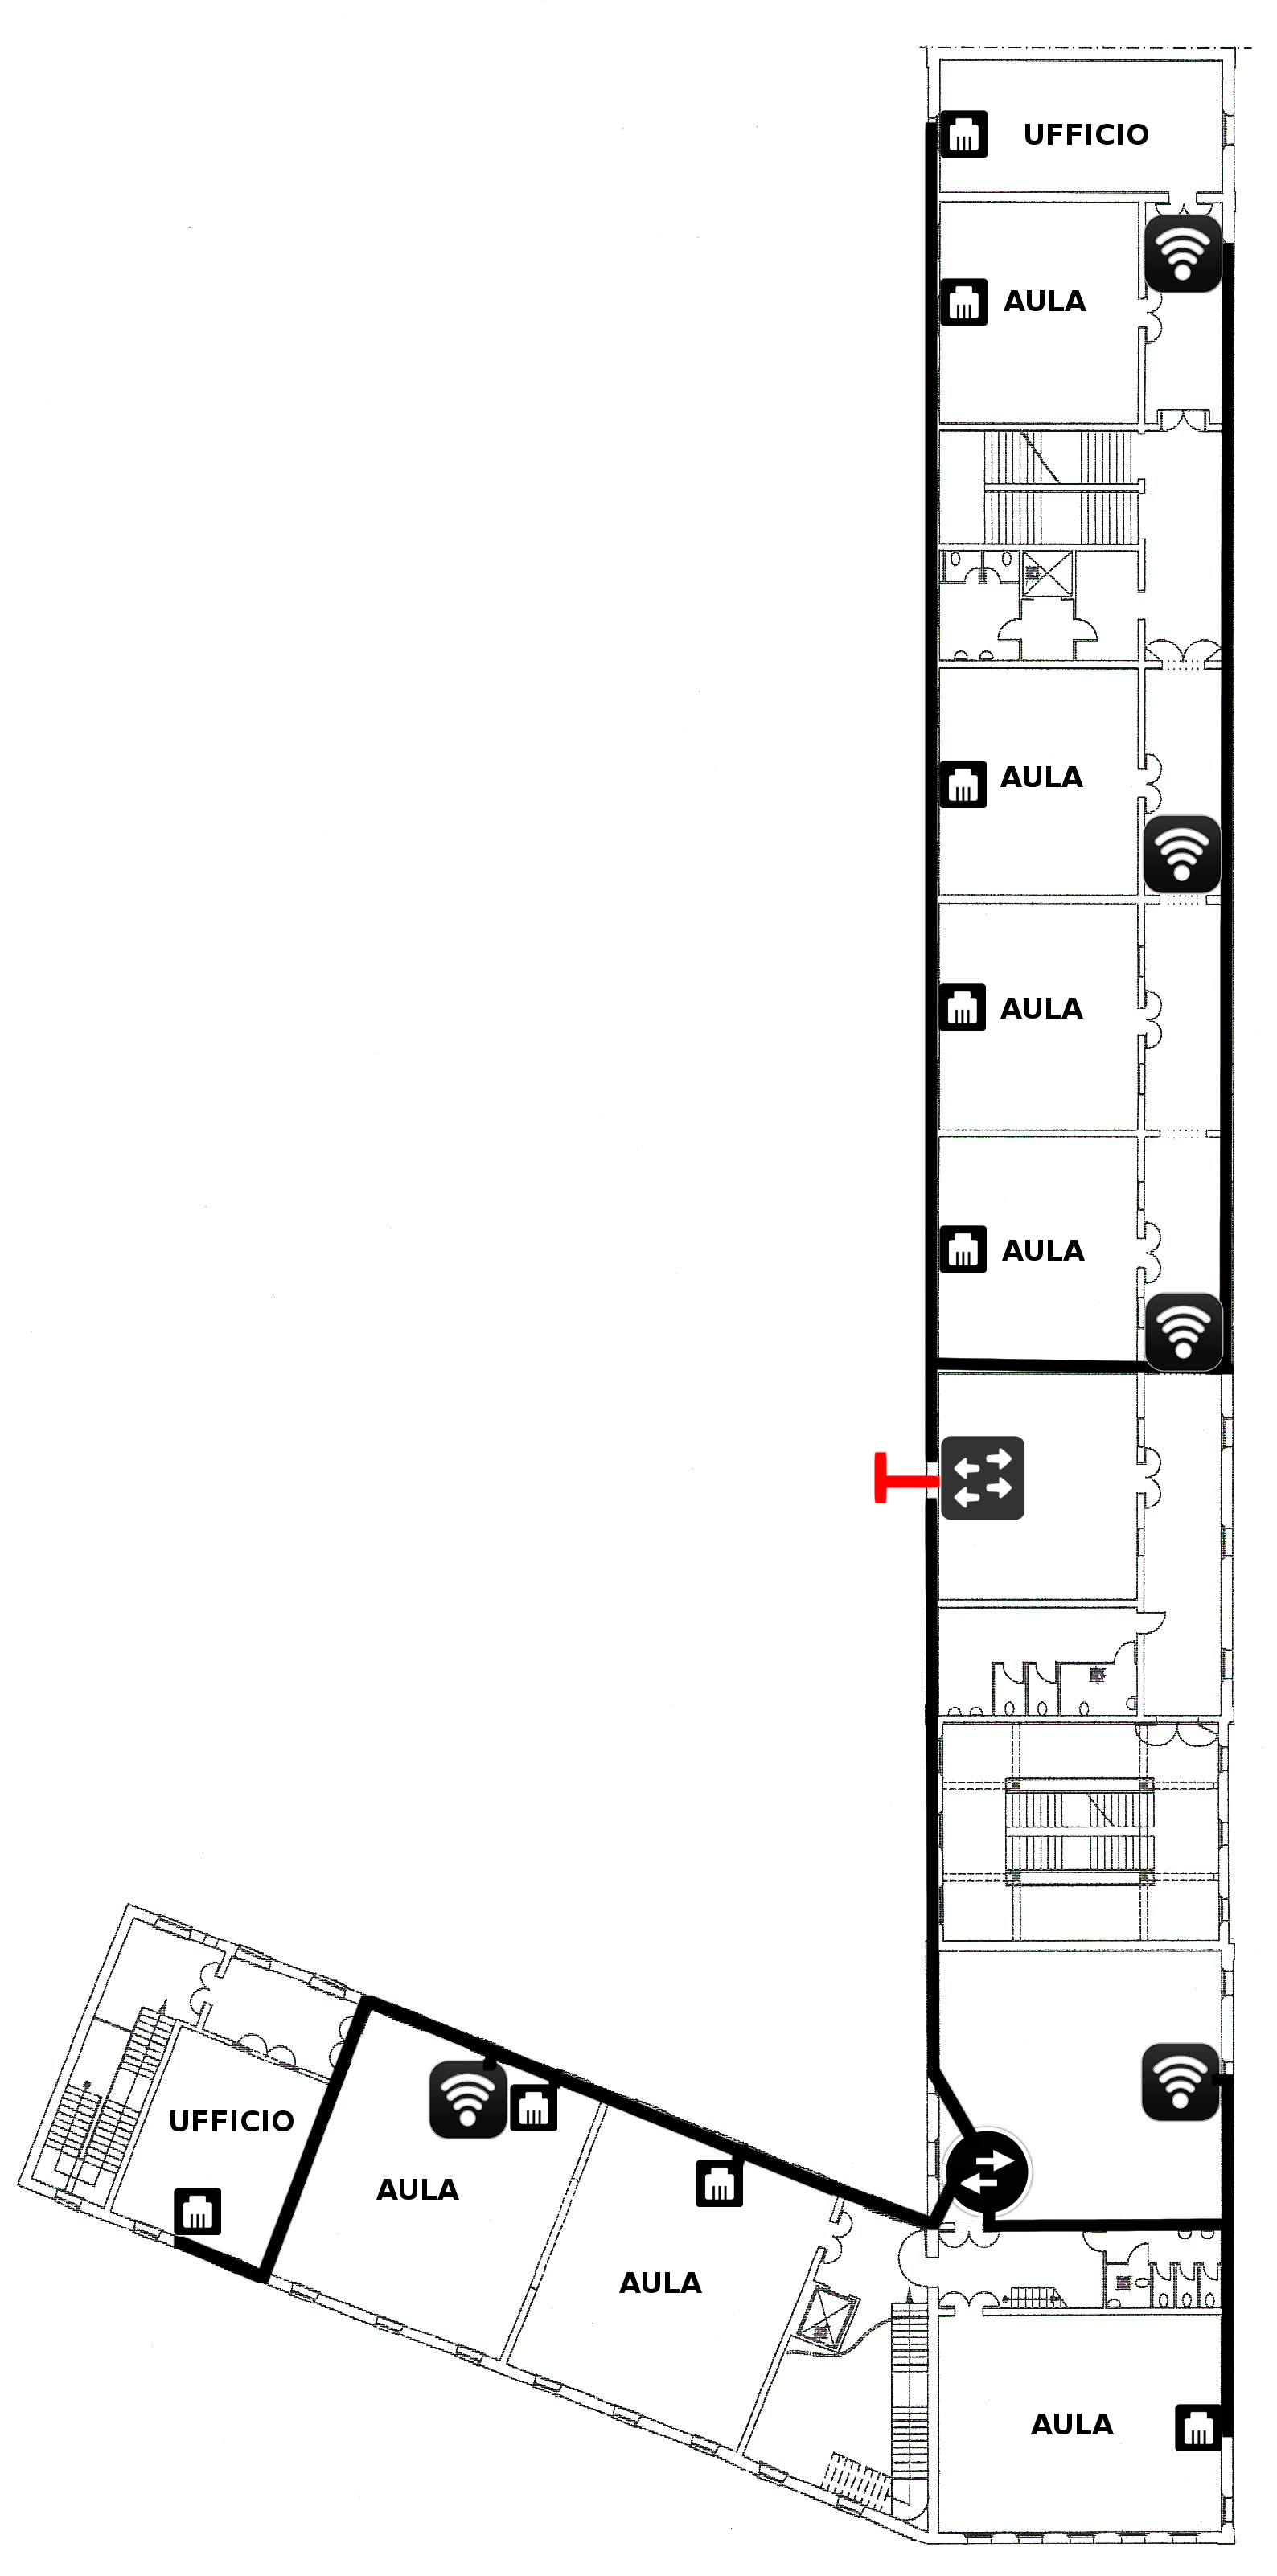
\includegraphics[scale=0.2]{architecture-002.png}
			\end{figure}
			\begin{figure}[H]
				\caption{Secondo piano, vecchio edificio}
				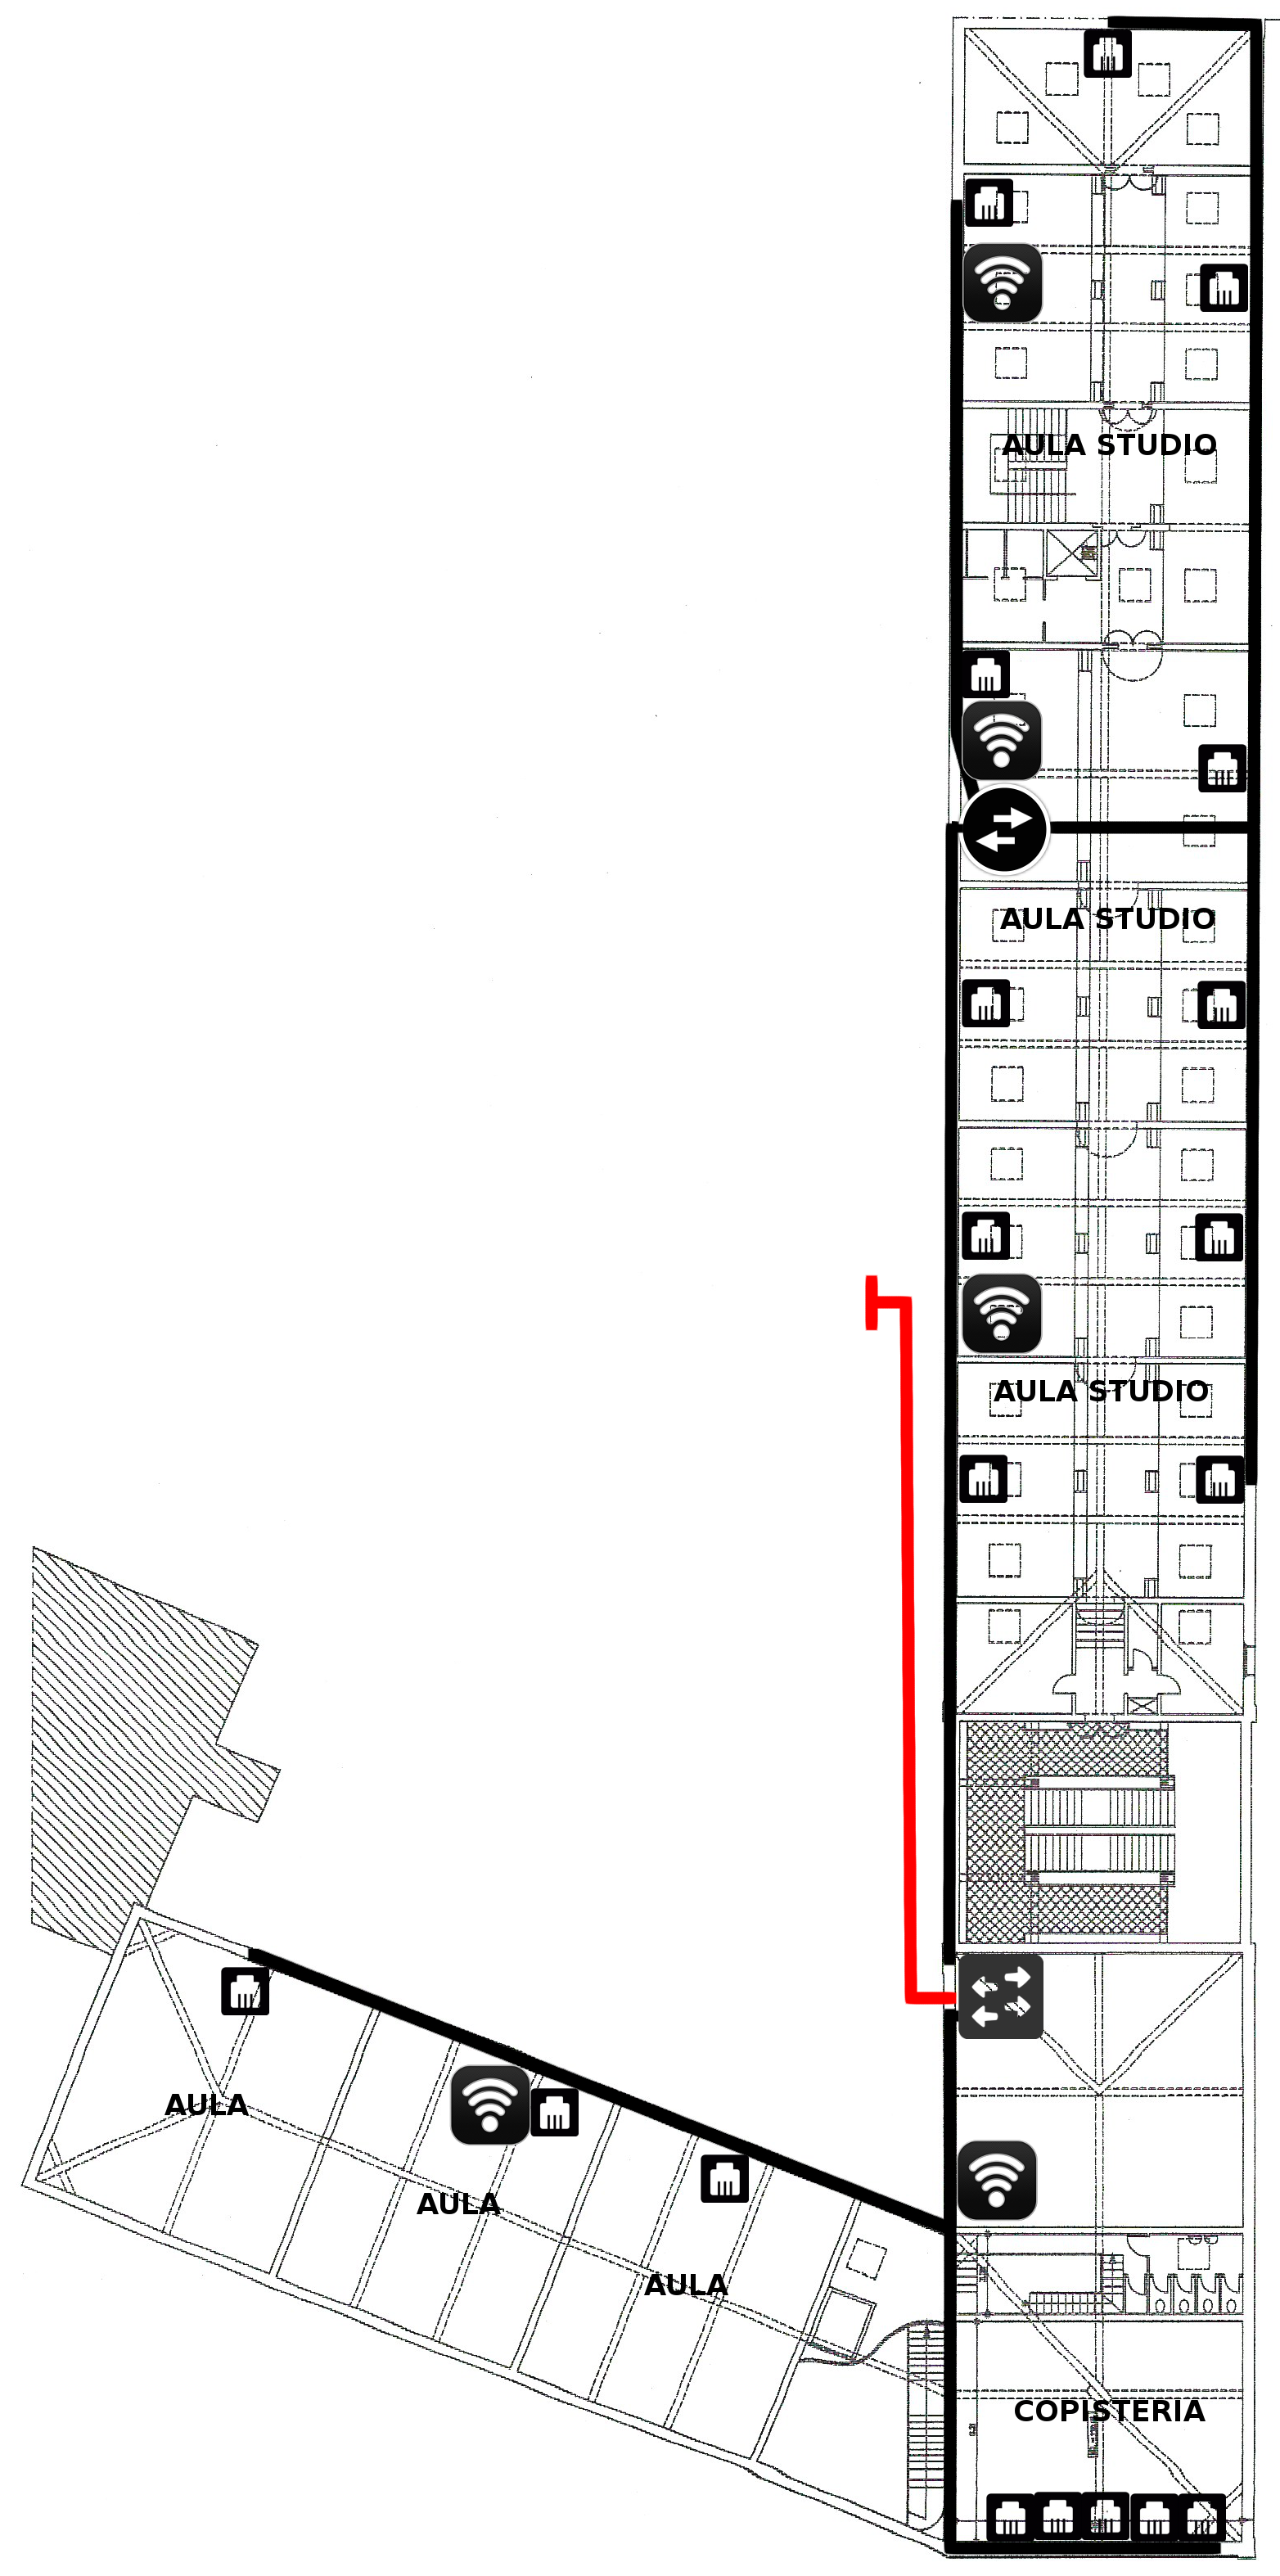
\includegraphics[scale=0.2]{architecture-003.png}
			\end{figure}
		\newpage
		\section{Nuovo edificio}
			\begin{figure}[H]
				\caption{Piano terra, nuovo edificio}
				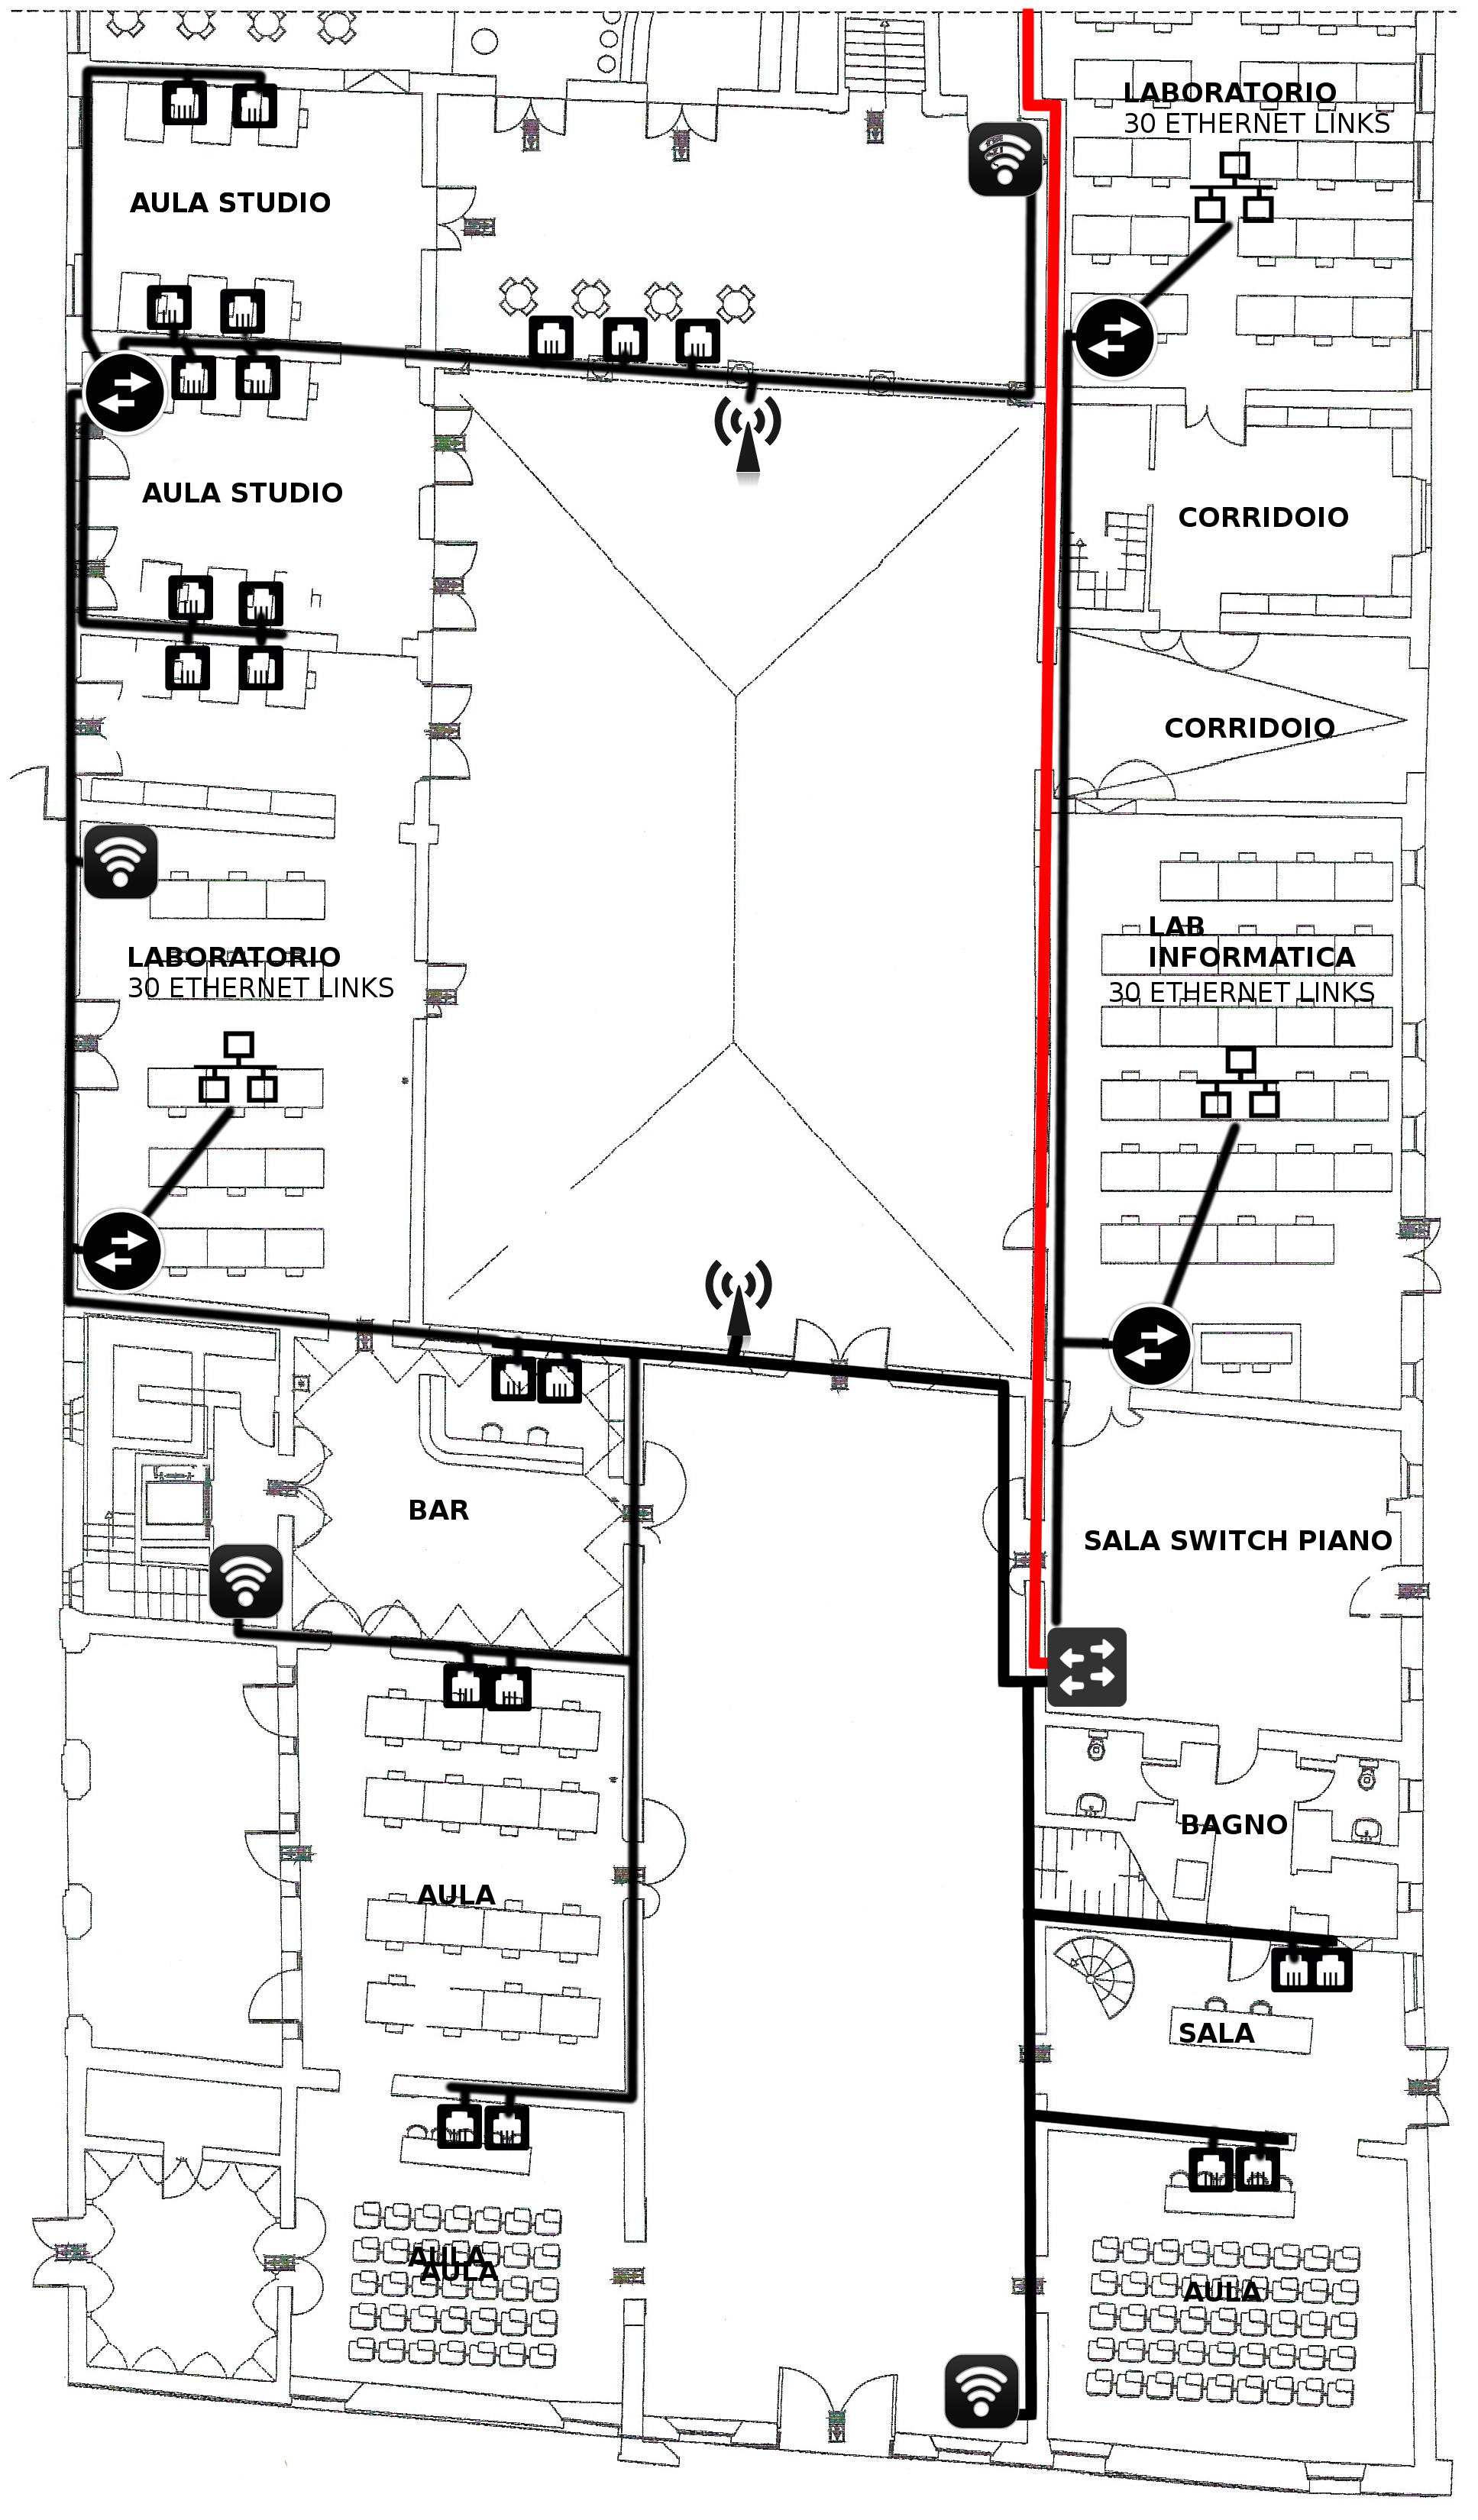
\includegraphics[scale=0.2]{architecture-004.png}
			\end{figure}
			\begin{figure}[H]
				\caption{Piano rialzato, nuovo edificio}
				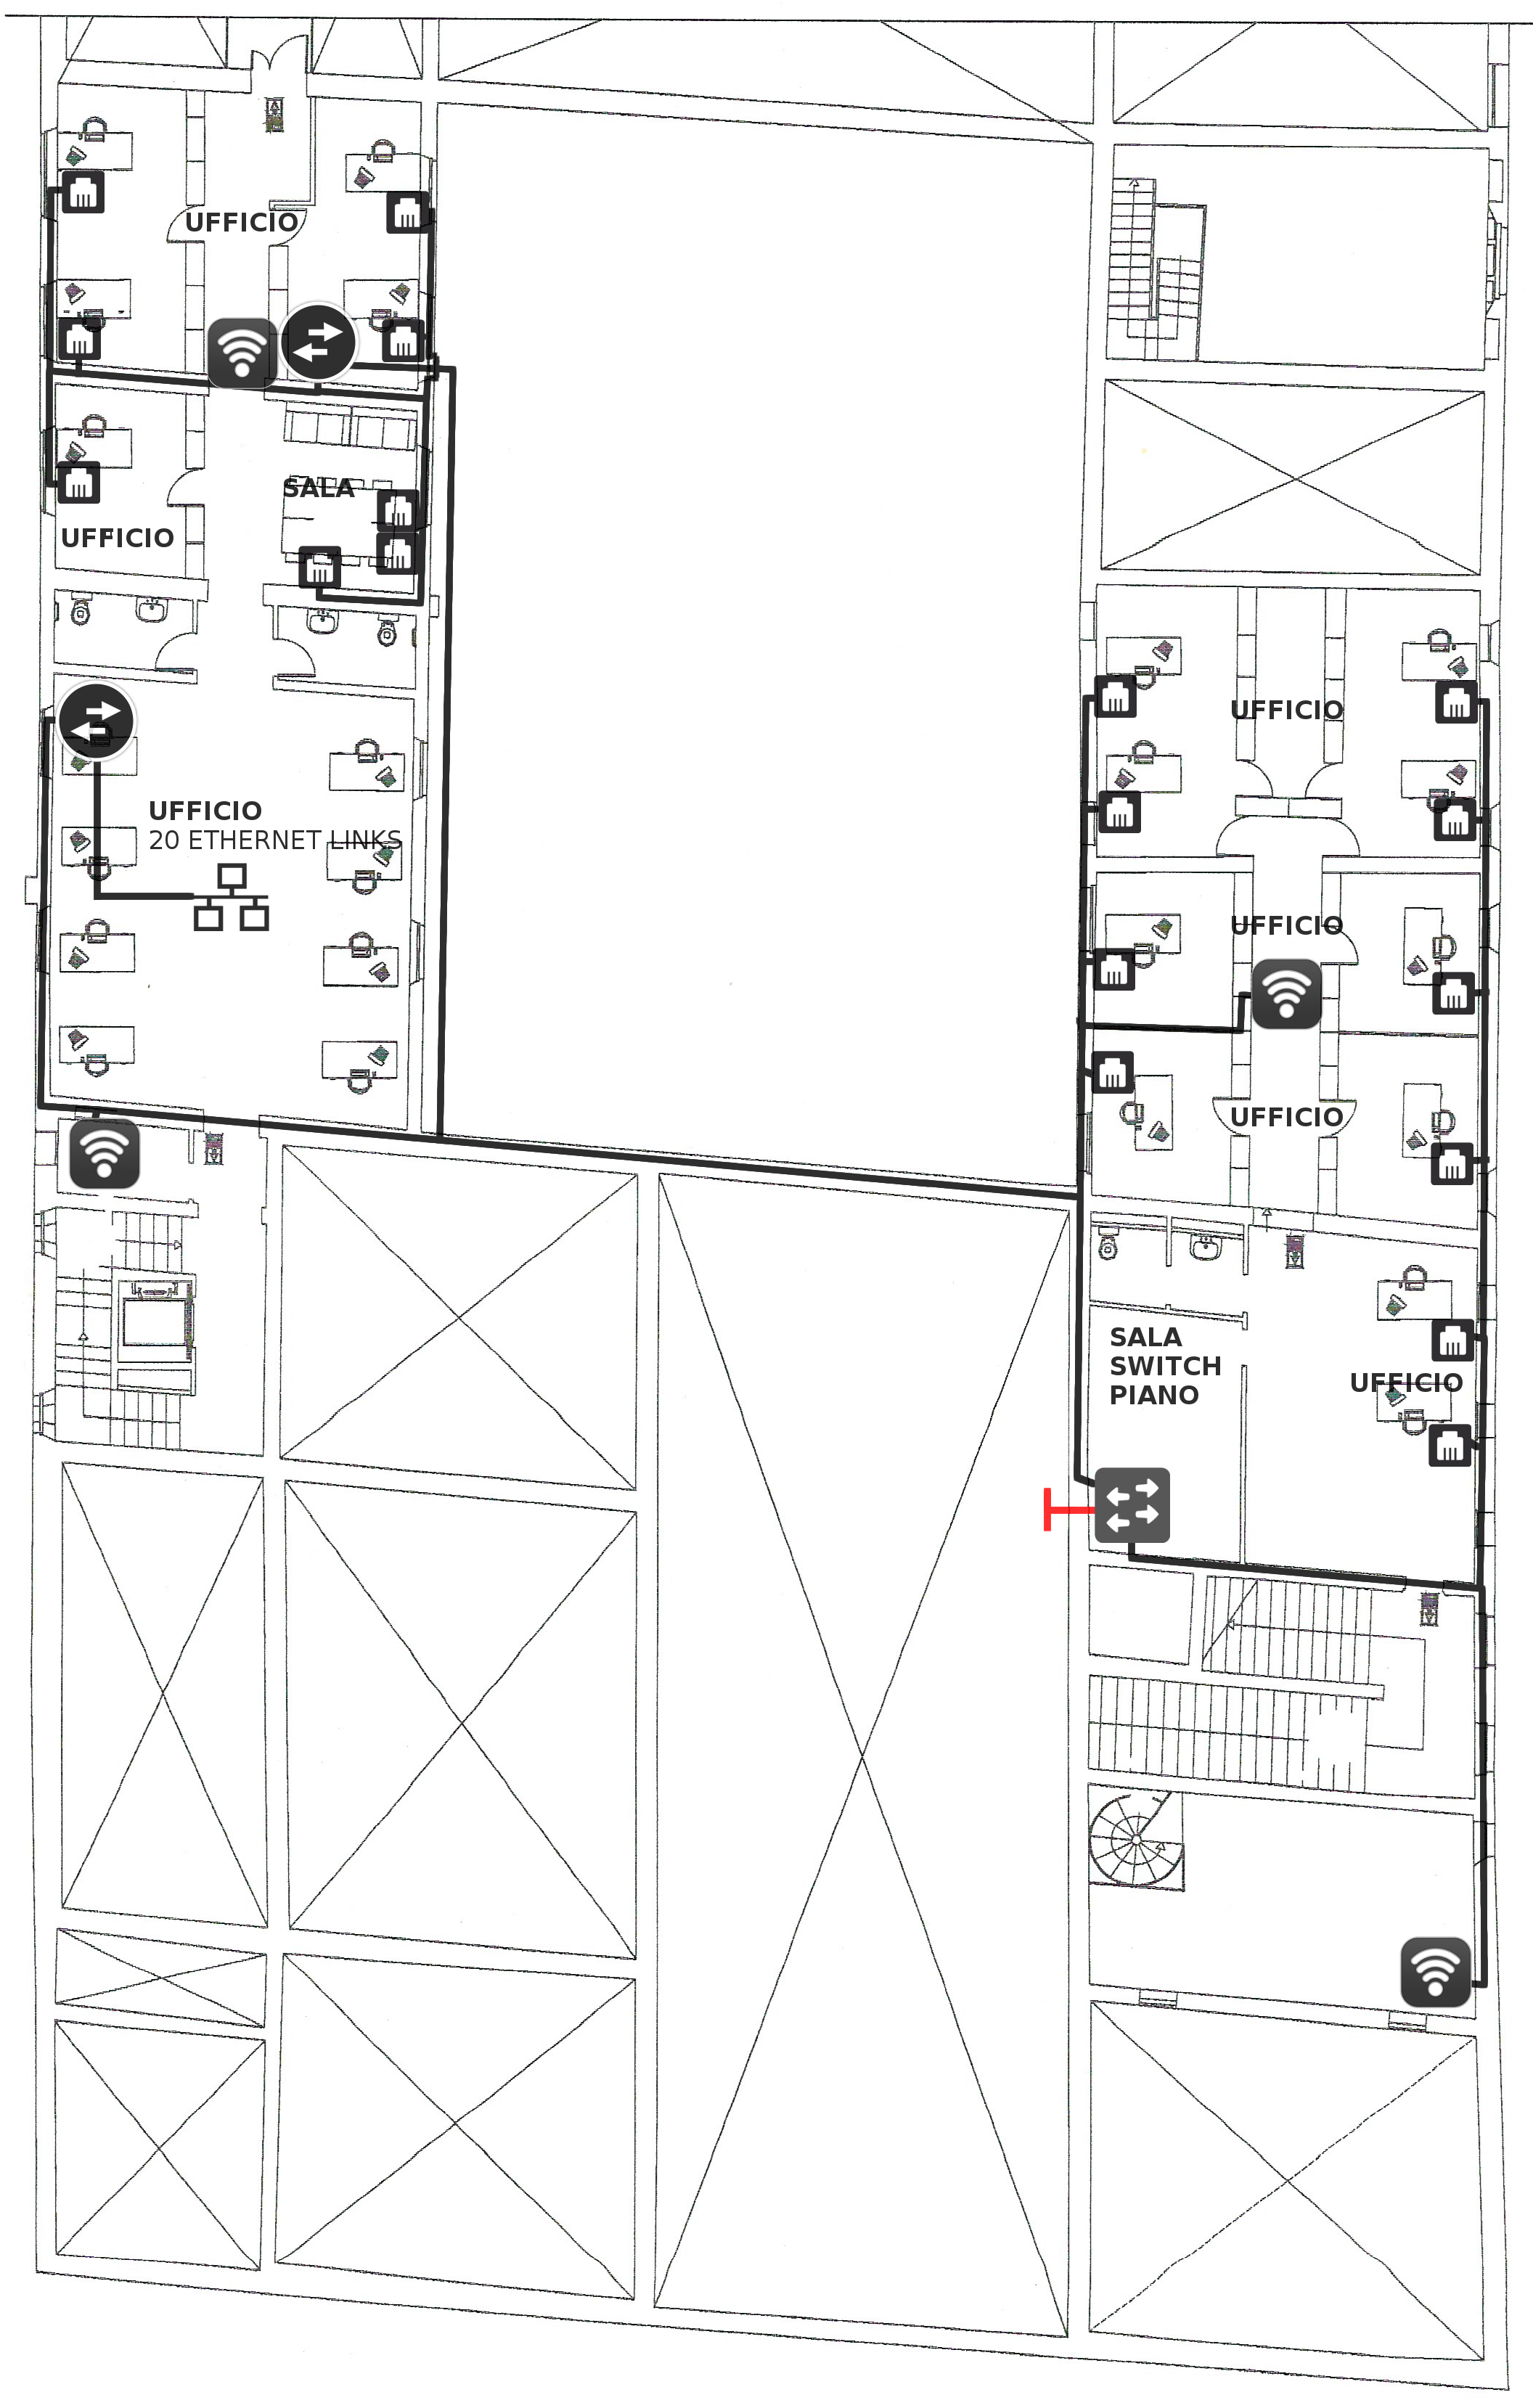
\includegraphics[scale=0.2]{architecture-005.png}
			\end{figure}
			\begin{figure}[H]
				\caption{Primo piano, nuovo edificio}
				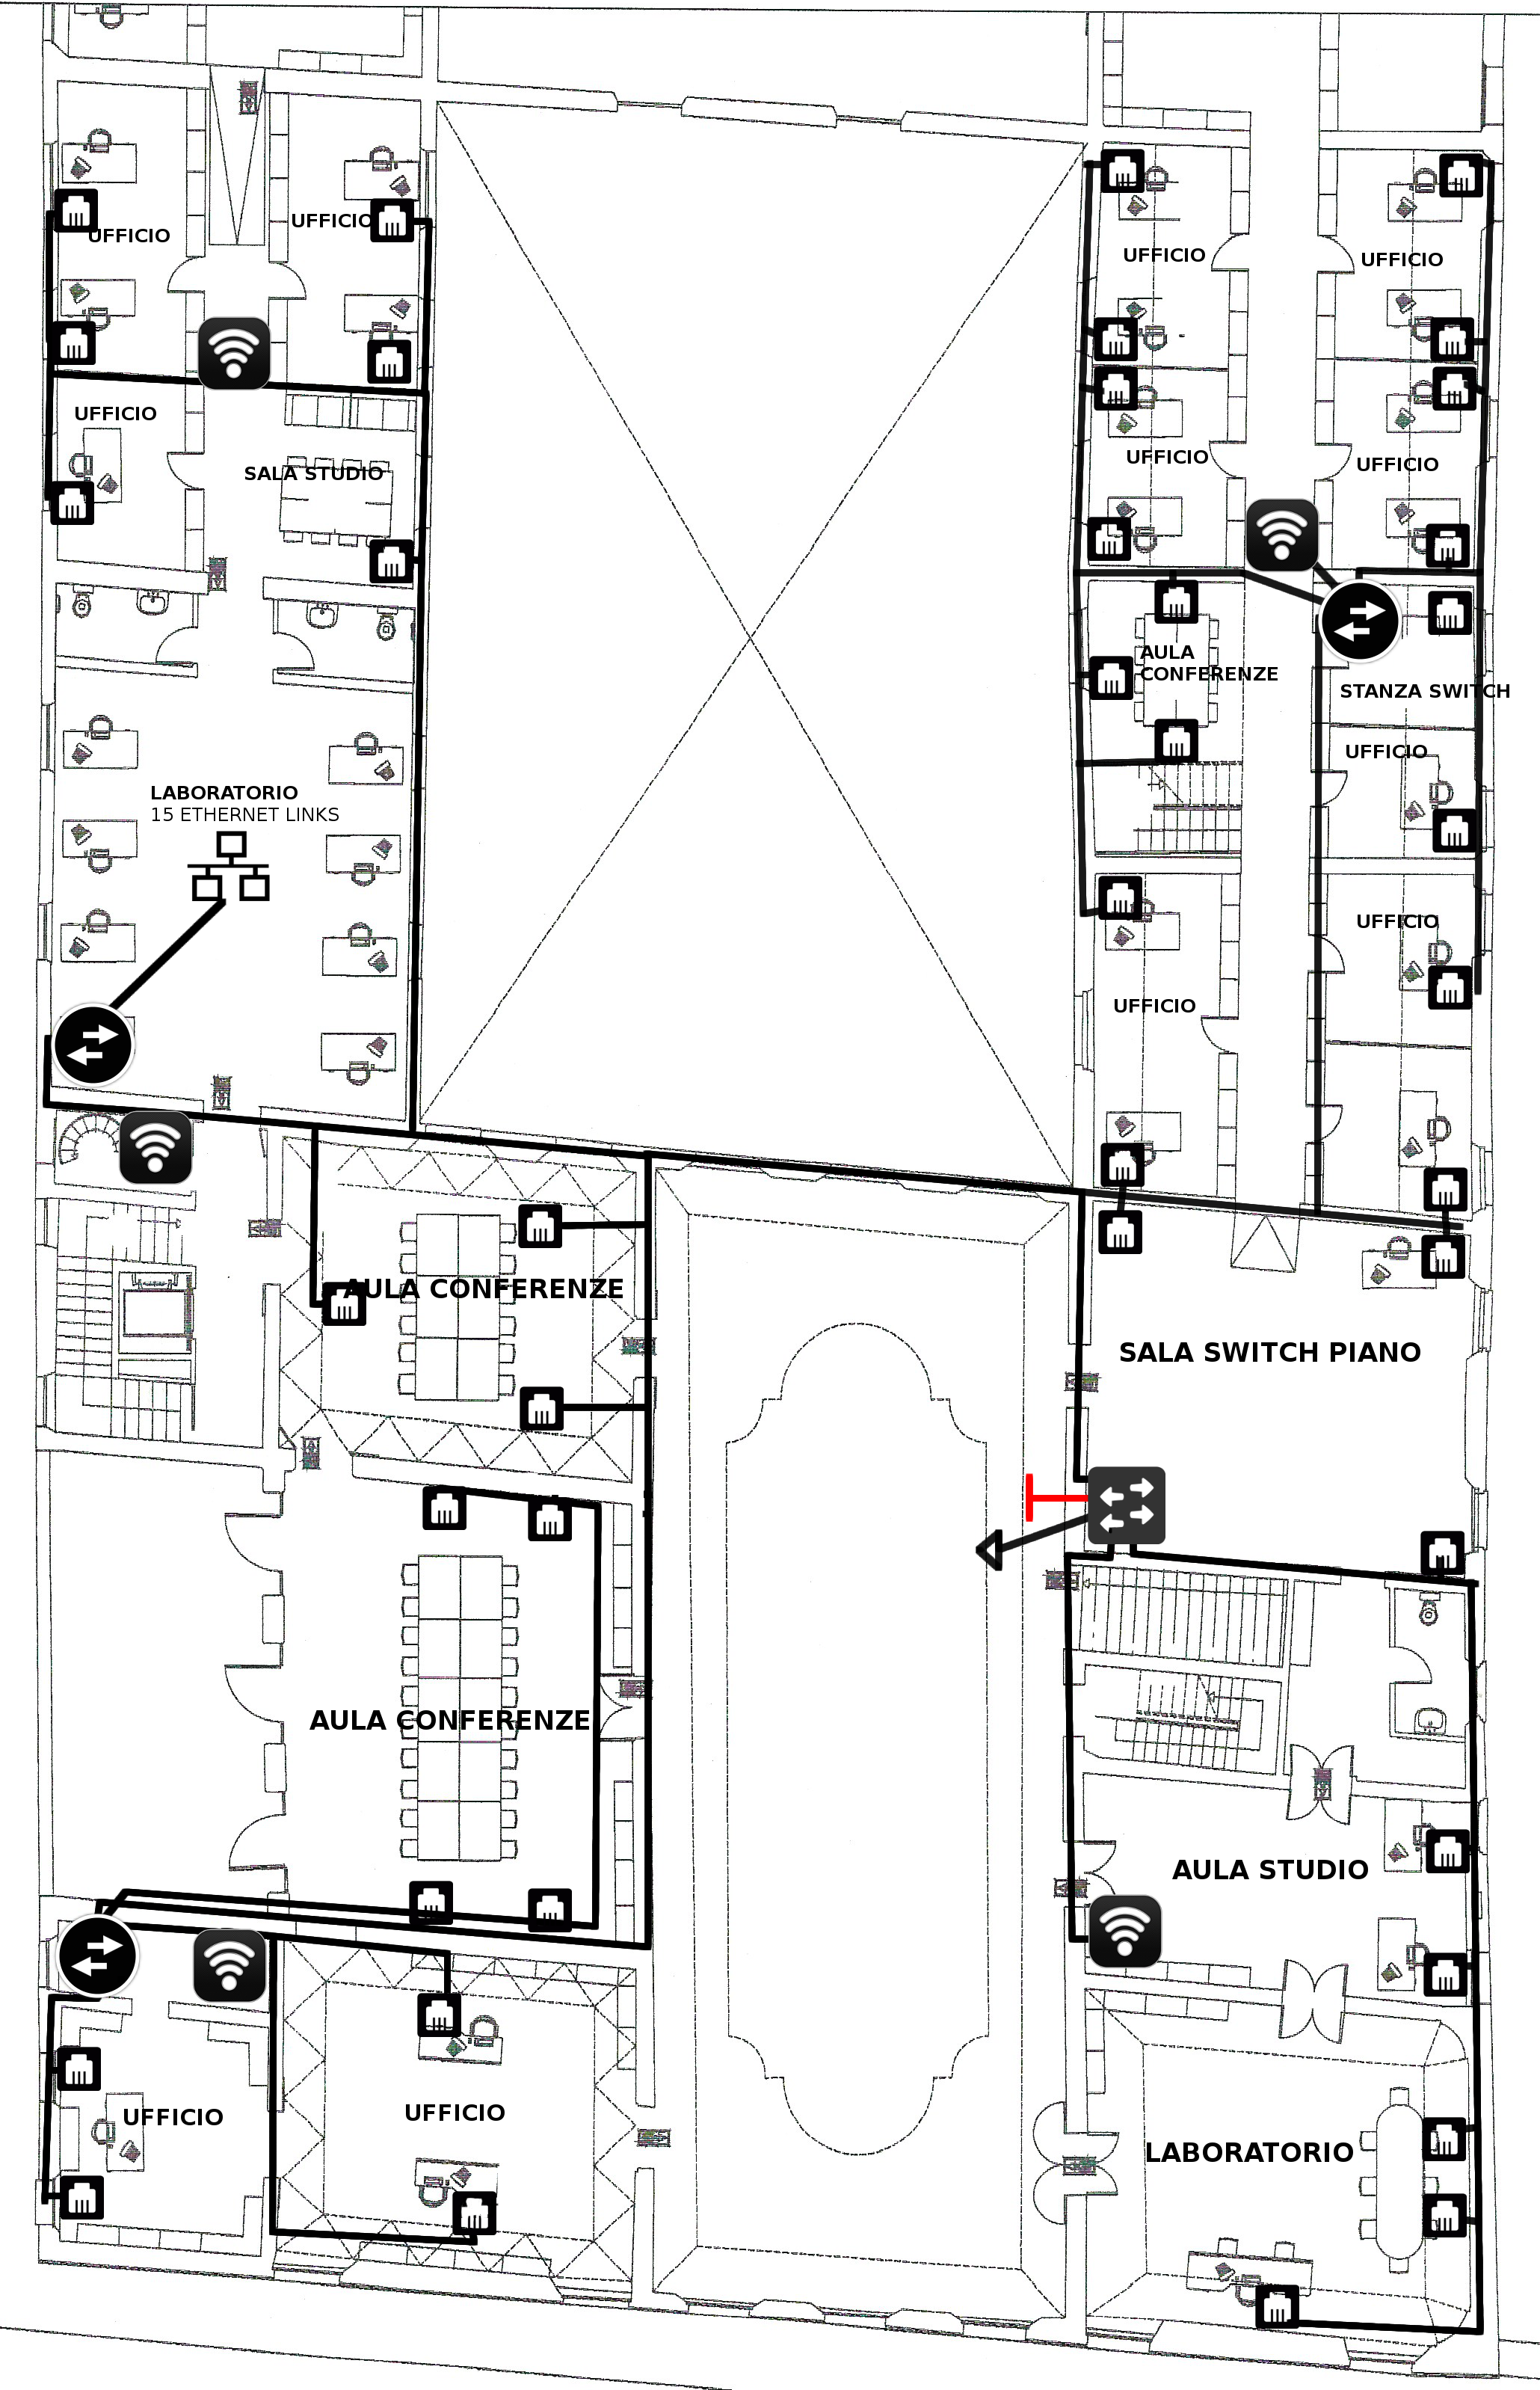
\includegraphics[scale=0.2]{architecture-006.png}
			\end{figure}
			\begin{figure}[H]
				\caption{Secondo piano, nuovo edificio}
				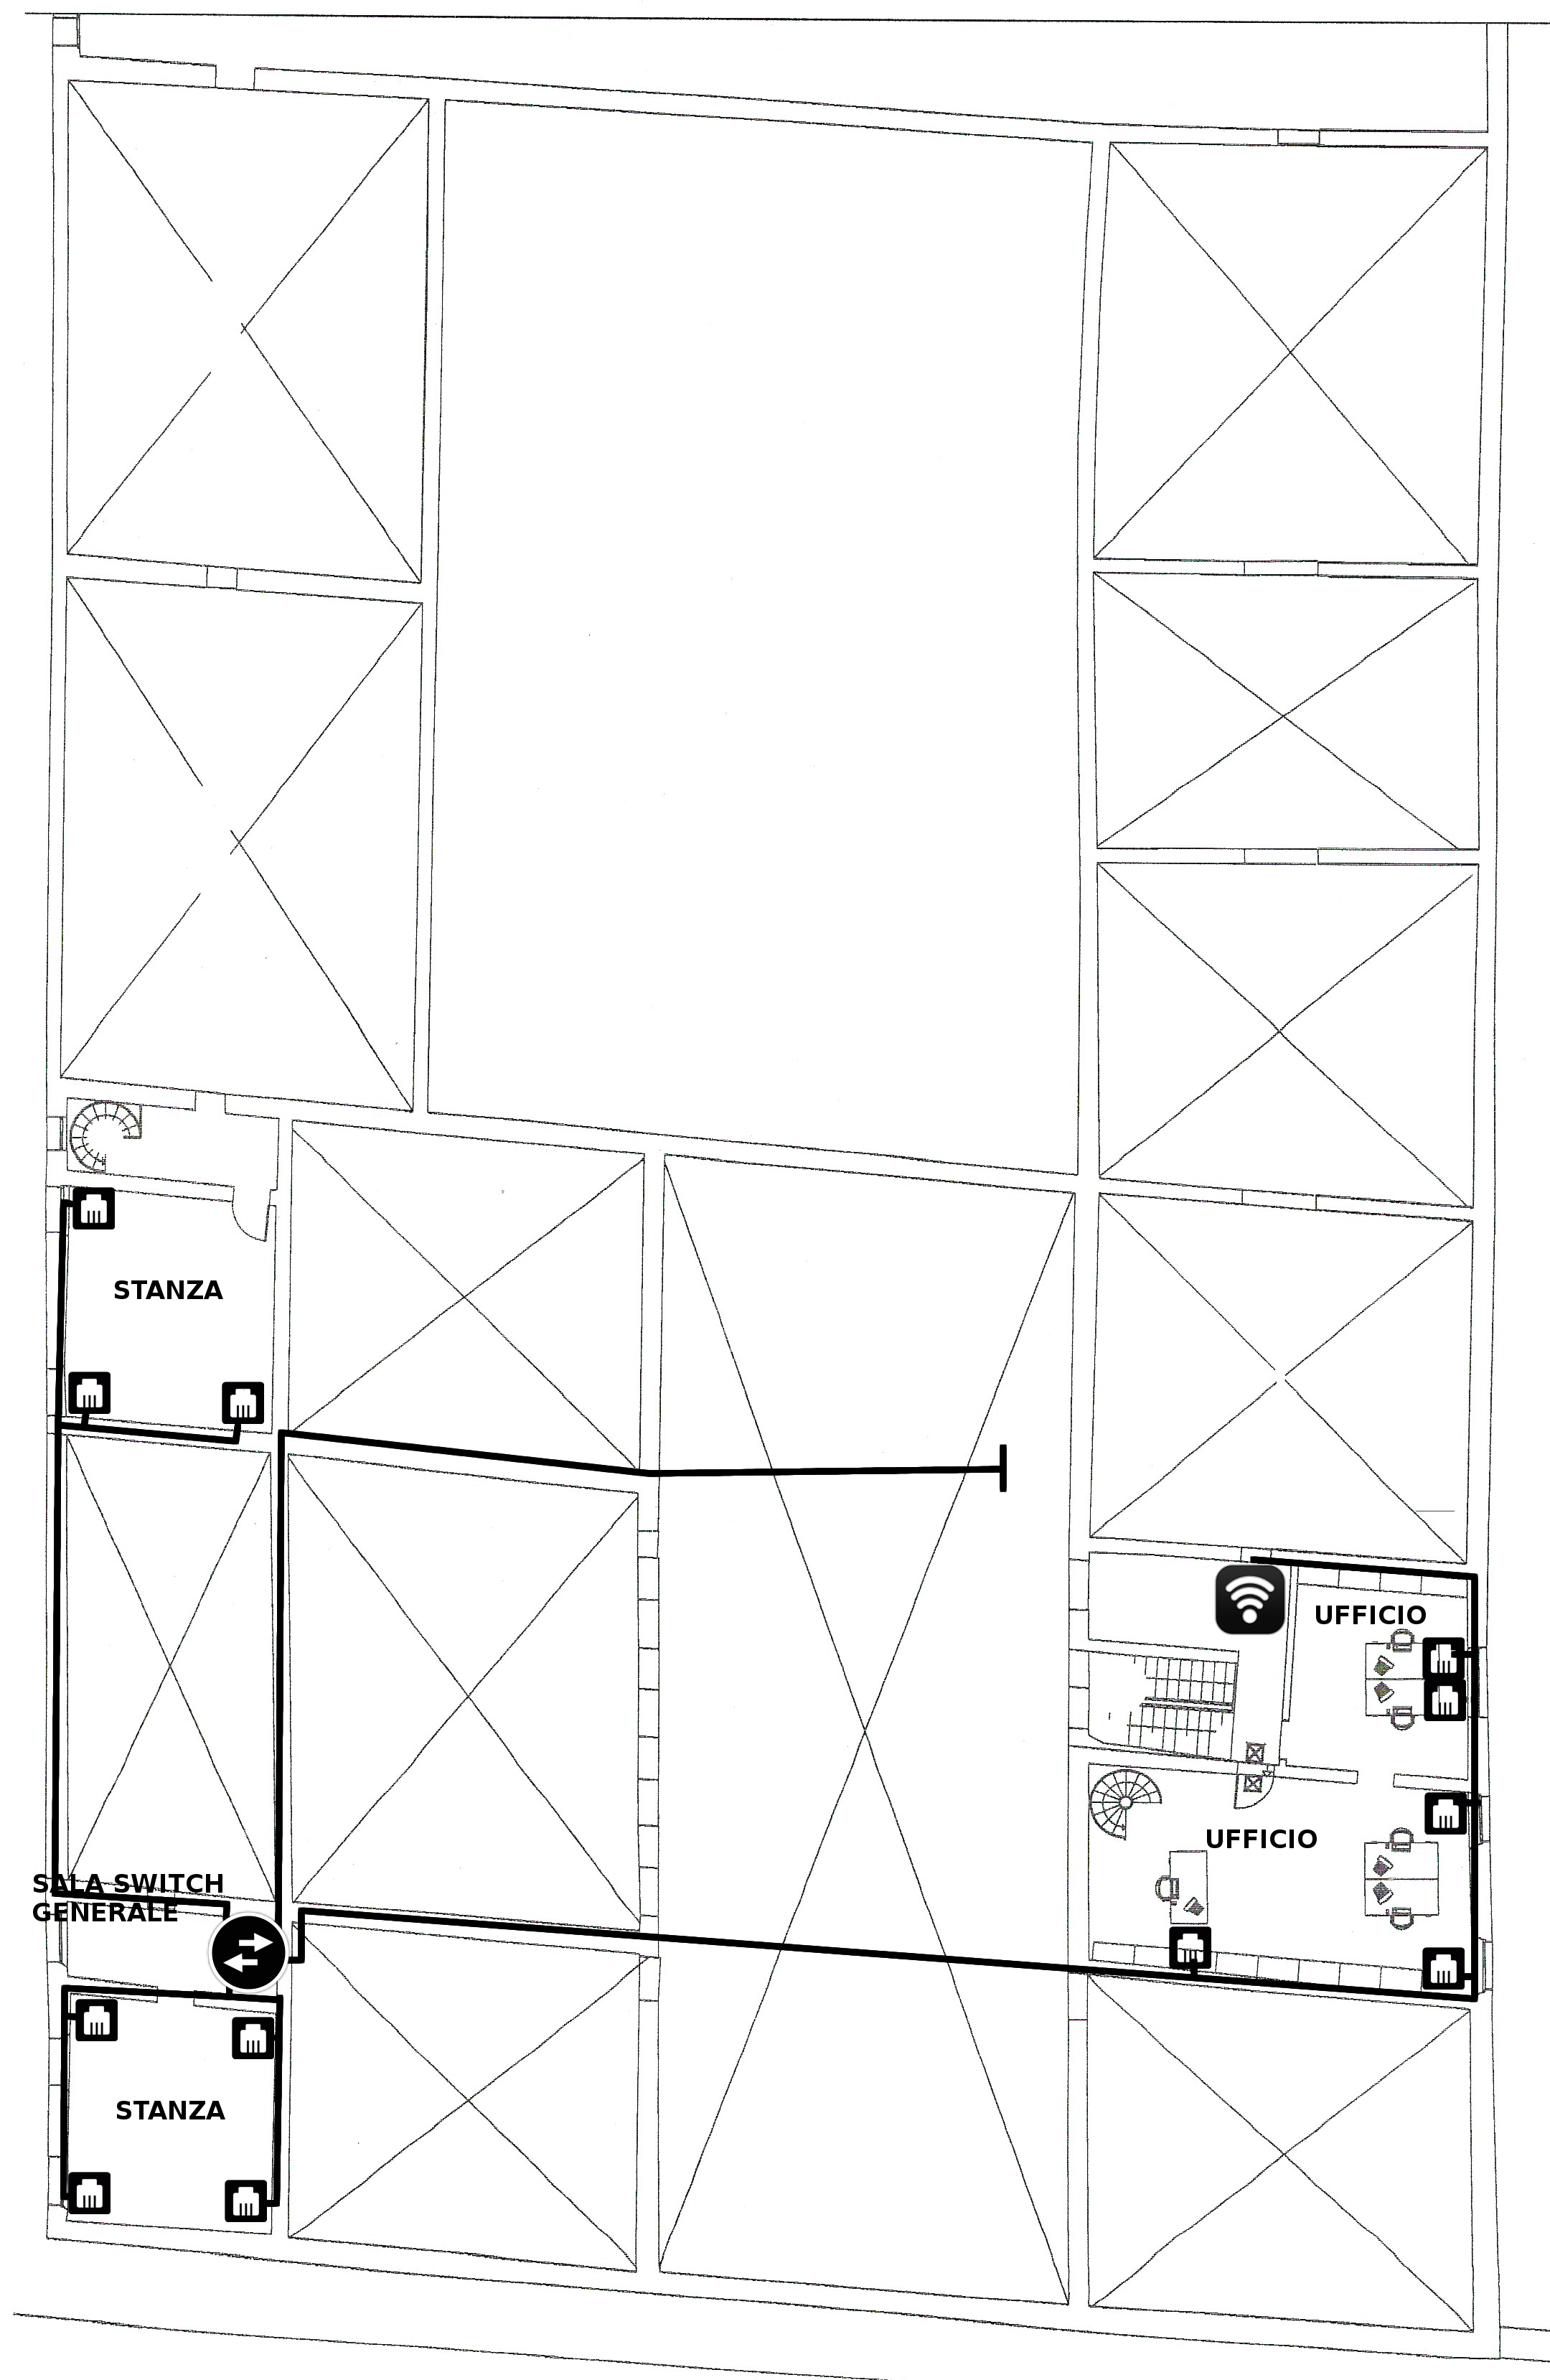
\includegraphics[scale=0.2]{architecture-007.png}
			\end{figure}
		
		\newpage
	\part{Preventivo}
		\begin{table}[h]
			\begin{tabular}{lrll}
				\hline
				\multicolumn{4}{c}{\textbf{Apparecchiature}} \\
				\cline{1-4}
				Prodotto & Prezzo (\euro{}) & Quantit\'a & Dove \\ \hline
				Cisco 3945E router & 7428.14 & 1 & Centro stella. \\
				Cisco WS-C4500X-32SFP+ switch & 7871.09 & 1 & Centro stella. \\
				Cisco Aironet 2702E-E-K9 & 784.46 & 30 & Ovunque. \\
				Cisco Aironet 1532E & 1196.87 & 2 & Esterni. \\
				Cisco WS-C3850-48U-S switch & 6370.00 & 6 & Switch di piano. \\
				HP J4904A 48-port Procurve & 815.28 & 13 & Switch locale. \\
				Tripp Lite SRW12US 12U rack & 280.81 & 19 & Rack per switch. \\
				APC Netshelter 44U & 383.84 & 1 & Rack centro stella. \\
				Sharp AEX12PHR clinatizzatore 3.5 kW & 2000.0 & 1 & Centro stella. \\
				TOT generale & 97764.64 \\
				\hline
			\end{tabular}
			\caption[Costo apparecchiature]{Stima dei costi delle apparecchiature}
		\end{table}
		
		\begin{table}[h]
			\begin{tabular}{lrl}
				\hline
				\multicolumn{3}{c}{\textbf{Materiali}} \\
				\cline{1-3}
				Prodotto & Prezzo (\euro{}/m) & Quantit\'a (m) \\ \hline
				Cavi in fibra multimodale bobina 300m & 740.0 & 4 \\
				Cavi in rame CAT 6a bobina 304m & 230.75 & 38 \\
				Frutti ethernet & 2.50 & 212 \\
				Teste cavo cat 6a (50 pz cad.) & 36.91 & 17 \\
				Materiale vario & 10000.00 \\
				TOT & 21665.97 \\
				\hline
			\end{tabular}
			\caption[Costo materiali]{Stima dei costi dei materiali}
		\end{table}

		\begin{table}[H]
			\begin{tabular}{lr}
				\hline
				\multicolumn{2}{c}{\textbf{Manodopera}} \\
				\cline{1-2}
				Servizio & Prezzo (\euro{}) \\ \hline
				Posa scatole ethernet & 2500.00 \\
				Posa cavi (fibra e rame) & 25000.00 \\
				Altro & 2500.00 \\
				TOT & 30000.00 \\
				\hline
			\end{tabular}
			\caption[Costo manodopera]{Stima dei costi della manodopera}
		\end{table}
		
		\par		
		TOTALE =  97764.64 \euro{} + 21665.97 \euro{} + 30000.00 \euro{} = 149170.61 \euro{}\newline
		TOTALE (sconto 45 \%) = \textbf{82043.84 \euro{}}
		
	
\end{document}
